\section{Assignment 1}

\begin{questions}

\question[5]
Consider the (first order, autonomous) ODE $f'(t)=f(t), f(0)=1$, and by using
uniform step sizes $\frac{1}{n}$ as done in class, write down an approximate
solution $f_n$, and show that $\forall t, f_n(t)$ goes to $e^t$ as $n$ goes to
infinity.  i did the case for $t=1$ in class (shown below). You're allowed to
assume the standard limit involving $e$ (that $\left( 1+\frac{x}{n}\right)^n$
goes to $e^x$ as n goes to infinity).



\begin{solution}
Consider $f' = f, f(0) = 1$. Approximate with step size of 1:
\begin{align}
f(1) &\approx f(0) + 1 f'(0) \\
     &= 1 + 1.1 = 2 \\
f(2) &\approx f(1) + 1f'(1) \\
     &= 2 + 1.2 = 4 \\
f(3) &\approx 4 + 1. f'(2) \\
	 &= 4 + 4 = 8 \\
     \vdots \\
f(n) &= 2^n  
\end{align}

Now we repeat it with step size of $\frac{1}{n}$.
\begin{align}
f(\frac{1}{n}) &\approx f(0) + \frac{1}{n} f'(0) \\
     &= 1 + \frac{1}{n} \\
f(\frac{2}{n}) &\approx f(\frac{1}{n}) + \frac{1}{n}f'(\frac{1}{n}) \\
     &= 1 + \frac{1}{n} + \frac{1}{n} \left( 1 + \frac{1}{n} \right) 
     	= \left( 1 + \frac{1}{n} \right) ^ 2\\
        \vdots \\
f(\frac{k}{n}) &= \left( 1 + \frac{1}{n} \right) ^k  
\end{align}

When $n$ becomes larger, our step size become smaller and smaller. When $k = n$
we have $f(\frac{n}{n}) = f(1) = \left( 1 + \frac{1}{n} \right)^n $. When $n
\rightarrow \infty, \left( 1 + \frac{1}{n} \right)^n \rightarrow e$.
\end{solution}

\question

In each of the four cases given, find the largest and the smallest
solution at $t=10$ among the four solutions for $y(0) 
= 1$, $y(1) = 1$, $y(-1)=1$, and $y(-1) = -1$.

\begin{align}
    \frac{dy}{dt} &= 5y \\
    \frac{dy}{dt} &= -3 y \\
    \frac{dy}{dt} &= 12y \\
    \frac{dy}{dt} &= -1.5y
\end{align}


\begin{solution}

All of these problem fall into $\frac{dy}{dt} = ky$ category.  It can be solved
easily.

\begin{align*}
    \frac{dy}{y} &= k dt \\
    \int \frac{dy}{y} &= \int k dt \\
    \ln y &=  k t + c 
\end{align*}

For each initial condition and value of $k$, we can calculate c to get the
solutions. For different initial conditions, the value of $c$ can be calculated
and more concrete expression of solution can be found.

\begin{enumerate}
    \item Case $y(0)$. $c = \ln y(0)  \implies \ln \frac{y}{y(0)} = kt \implies
        y = y(0) e^{kt} $
    \item Case $y(1)$. $c = \ln y(1) - k  \implies \ln \frac{y}{y(1)} = k(t-1)
        \implies y = y(1) e^{k(t-1)} $
    \item Case $y(-1)$. $c = \ln y(-1) - k  \implies \ln \frac{y}{y(1)} = k(t+1)
        \implies y = y(-1) e^{k(t+1)}$
\end{enumerate}

Figure \ref{fig:problem2} shows the numerical solutions using python-numpy.
Script is available \href{put link here}{put link here}. The output of script
shows the values: in two cases values are too close to zero to make a
difference between min and max. One can analytically determine the min and max. 

\begin{verbatim}
Case :-1.5
	 Init     (1, 0)  y(10) = (3.01360478337e-07+0j)
	 Init     (1, 1)  y(10) = (1.35059765221e-06+0j)
	 Init    (1, -1)  y(10) = (6.72432835558e-08+0j)
	 Init   (-1, -1)  y(10) = (-6.72432835558e-08+0j)
Case :12
	 Init     (1, 0)  y(10) = (1.47045343317e+52+0j)
	 Init     (1, 1)  y(10) = (9.03478277055e+46+0j)
	 Init    (1, -1)  y(10) = (2.39323225334e+57+0j)
	 Init   (-1, -1)  y(10) = (-2.39323225334e+57+0j)
Case :5
	 Init     (1, 0)  y(10) = (5.45052316477e+21+0j)
	 Init     (1, 1)  y(10) = (3.67253437758e+19+0j)
	 Init    (1, -1)  y(10) = (8.08929194814e+23+0j)
	 Init   (-1, -1)  y(10) = (-8.08929194814e+23+0j)
Case :-3
	 Init     (1, 0)  y(10) = (2.1030205942e-13+0j)
	 Init     (1, 1)  y(10) = (3.06022787369e-12+0j)
	 Init    (1, -1)  y(10) = (5.91407220526e-13+0j)
	 Init   (-1, -1)  y(10) = (-5.91407220526e-13+0j)
\end{verbatim}

\end{solution}

\begin{figure}[h!]
    \includegraphics[width=\textwidth]{./problem2_solution.png}
    \caption{Solution to problem 2. $t = 0$ to $t = 10$. }
    \label{fig:problem2}
\end{figure}



\question[5]
\label{prob3}

For a certain microorganism, birth is by budding off a fully copy of itself.
Suppose that under reasonable favorable laboratory conditions (plenty of food
and no predation), such birth occurs on average four times per day, and an
individual lives, on average, one day. Write a differential equation for the
population, $p(t)$, of the microorganism as a function of time. Then find the
solution given that at time zero, the population numbered 1000.



\begin{solution}

This problem is simple as far as mathematics is concerned.  Each individual
goes through a birth event 4 times a day, and death event 1 time per days.
Effectively, this leaves us with 3 birth events per day per individual. Here
the unit of time is "day" (which is infinitely small only when we consider
time-scale of evolution).

\begin{align}
\frac{dp(t)}{dt} &= 4 p(t) - p(t) = 3 p(t) \\
p(t) &= k e^{3t}
\end{align}

Now we use the initial condition $p(0) = 1000$ to find the solution : $ p(t)  = 1000e^{3t} $.

\end{solution}

\question
    Think about problem 6. No need to hand in.


\question[5]
\label{problem5}
    $\frac{dp}{dt} = (p-1)(p-2)$. Sketch graphs of $p(t)$ versus $t$ for
    solutions with

    \begin{enumerate}
        \item $ p(0) = -1 $
        \item $ p(0) = 1/2 $
        \item $ p(0) = 2 $
    \end{enumerate}

\begin{solution}

The solution is $p(t) = \frac{ke^t-2}{ke^t -1} $. The value of $k$ depends on
given initial conditions. The figure \ref{fig:problem5} shows the solutions. The
python script can be found in appendix.

\end{solution}

\begin{figure}[htpb]
    \centering
    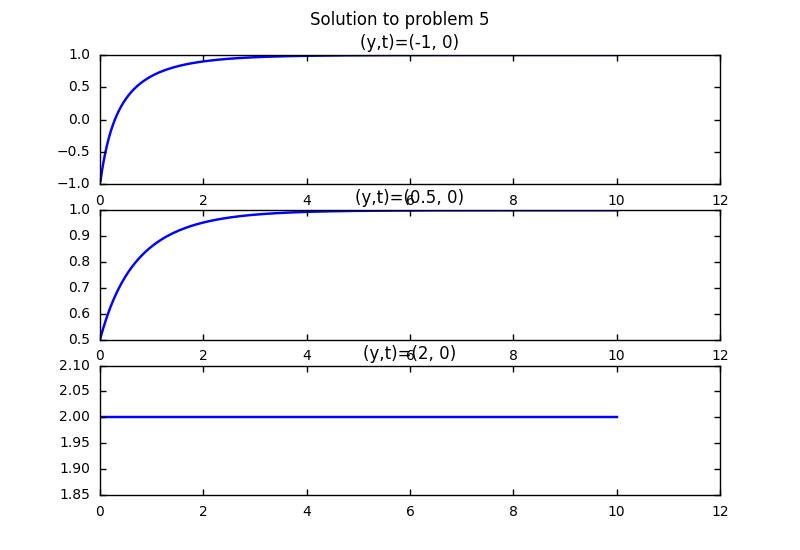
\includegraphics[width=0.8\linewidth]{./solve_problem5_py.png}
    \caption{Solution to \ref{problem5}}
    \label{fig:problem5}
\end{figure}

\question[5]
\label{problem6}

$\frac{dp}{dt} = 1 - e^p$. Sketch graphs of $p(t)$ versus $t$ for solutions
with 
\begin{enumerate}
    \item $p(0) = -1 $
    \item $p(0) = 1 $
    \item $p(0) = 4 $
\end{enumerate}

\begin{solution}

    This system was solved with python-numpy. The solution for each case is
    shown below in figure \ref{fig:problem6}.

    My analytical solution

    \begin{align*}
        \frac{dp}{dt} &= 1 - e^p \\
        \frac{dy}{y(1-y)} &= dt && \text{Substitute $e^p=y, \; e^p dp = dy $. } \\
        \ln y - \ln (1-y) &= t + c && \text{Solve for y.} \\
        \ln \frac{y}{1-y} &= t + c \\
        \frac{y}{1-y} &= e^{t+c} \\
        \frac{e^p}{1-e^p} &= ke^t && \text{Substitute $y=e^p$ and $e^c=k$ } \\
    \end{align*}

    One can further simplify it. The sanity check would to be differentiate it
    and see if it matches the original equations.

\end{solution}

\begin{figure}[htpb]
    \centering
    \includegraphics[width=0.8\linewidth]{./solve_problem6_py.png}
    \caption{Solution to problem \ref{problem6}. For different initial
    condition, this system is either growing or decaying! }.
    \label{fig:problem6}
\end{figure}

    

\question[5]
\label{pb1:graphs}

Suppose the function $x(t)$ evolves according to a differential equation:
$\frac{dx}{dt} = f(x)$. For each of the four candidate functions $f(x)$
graphed in figure \ref{fig:graphs}, describe what happens to $x(t)$ as $t$
gets large if $x(0) = 1$.

\begin{figure}[htpb]!
    \centering
    \includegraphics[width=0.8\linewidth]{./graphs.pdf}
    \caption{$y(x)$ for problem \ref{pb1:graphs}. }
    \label{fig:pb1_graph}
\end{figure}

\begin{solution}
    
    To be able to use numerical engine I have been using, I need concrete value
    of $y(x)$ so I regenerated these graphs using scale and pencil. Since
    y-values are not given, I simply took the scale value in millimeter.  The
    shape of $f(x)$ matches the original graphs approximately. The result are
    shown in figure \ref{fig:solve_pb1_graph}.
    
\end{solution}

\begin{figure}[htpb]
    \centering
    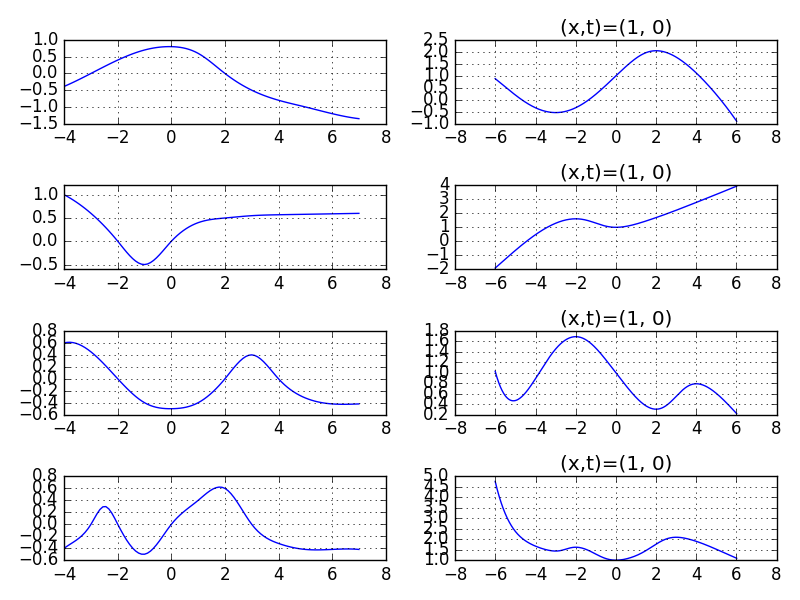
\includegraphics[width=\linewidth]{./solve_problem7_py.png}
    \caption{Solution to problem 8. On the left we have $y(x)$, on the right, we
    have solution to the system $\frac{dy}{dx} = y(x)$  with given initial
    condition $y(0) = 1 $.}
    \label{fig:solve_pb1_graph}
\end{figure}

\question[5]
\label{pb2:graphs}

    For each of the same four functions as in problem \ref{pb1:graphs}, describe
    what happens to $x(t)$ as $t$ gets large if $x(0) = -4 $.
    

    \begin{figure}[htpb]
        \centering
        \includegraphics[width=\linewidth]{./solve_problem8_py.png}
        \caption{Solution to problem 7. On the left we have $y(x)$, on the right, we
            have solution to the system $\frac{dy}{dx} = y(x)$  with given initial
            condition $y(0) = -4 $. Compared to previous result, the shape do not
            change; only there is negative shift in y-axis. 
        }
        \label{fig:pb2_graph}
    \end{figure}


\question[5]
For each of the four functions in problem \ref{pb1:graphs}, list the
equilibrium points and decide which are stable and which are unstable. 

\begin{solution}

    If a system reaches to the equilibrium point, it solution is constant
    for all the time. If it is a stable equilibrium point, then it tends to come
    back to equilibrium point if perturbed. If it is in unstable equilibrium point, 
    a small perturbation would be enough it make the system go to some other
    state. For a point to be equilibrium, the rate of change of system state at
    that point must be zero.

    For each cases wherever $y(x) = 0$, is a equilibrium point. Point $x=-3,2$,
    $x=-2,0$, $x = -2, 2, 4$, and $x=-3,-2,0,$ are equilibrium point. To
    establish if the point is also stable, one needs to do bit more: check the
    rate of change to the left of right direction of the point. Draw and arrow
    which shows the direction of change at that point at both side. A stable
    equilibrium point has $ \rightarrow .  \leftarrow $ profile.

    Convince yourself that when $\frac{df}{dx}$ (which is $y(x)$ in this case)
    has a negative slope at equilibrium point, then it is a stable equilibrium.
    
\end{solution}

\end{questions}

